\section{Results}
\label{sec:results}

\subsection{Perplexity Sensitivity by Axis}
\label{sec:main_results}

\Tabref{tab:main_results} presents the core results for \qwenseven. Four of five pragmatic axes show statistically significant directional preferences after Bonferroni correction.

\begin{table}[t]
    \centering
    \caption{Perplexity sensitivity results for \qwenseven across 30 scenarios. $\dloglik$: mean signed log-likelihood difference (positive = prefers Pole~B). Consistency: $|2f{-}1|$ where $f$ is the fraction preferring the majority pole. All $p$-values are Bonferroni-corrected ($\alpha{=}0.0083$). Best (largest) effect sizes among pragmatic axes in \textbf{bold}.}
    \resizebox{\textwidth}{!}{%
    \begin{tabular}{@{}lrrlrrrrl@{}}
        \toprule
        \textbf{Axis} & \textbf{Mean $\dloglik$} & \textbf{\% Pole~B} & \textbf{Preferred} & \textbf{Consistency} & \textbf{Sign $p$} & \textbf{Wilcoxon $p$} & \textbf{Cohen's $d$} & \textbf{Sig.?} \\
        \midrule
        Politeness   & $+0.851$ & 96.7\% & polite   & \textbf{0.933} & $<$0.001 & $<$0.001 & \textbf{$+1.81$} & YES \\
        Specificity  & $-0.374$ & 13.3\% & vague    & 0.733 & $<$0.001 & $<$0.001 & $-1.02$ & YES \\
        Directness   & $-0.313$ & 20.0\% & indirect & 0.600 & 0.001    & $<$0.001 & $-0.94$ & YES \\
        Formality    & $+0.234$ & 76.7\% & formal   & 0.533 & 0.005    & 0.001    & $+0.68$ & YES \\
        Emot.\ tone  & $-0.033$ & 46.7\% & ---      & 0.067 & 0.856    & 0.459    & $-0.08$ & no \\
        \midrule
        Synonym (ctrl) & $-1.057$ & 0.0\% & version A & 1.000 & $<$0.001 & $<$0.001 & $-3.26$ & --- \\
        \bottomrule
    \end{tabular}
    }
    \label{tab:main_results}
\end{table}

\para{Politeness} is the strongest pragmatic variable under consideration. The model prefers polite responses in 96.7\% of scenarios ($d{=}1.81$), with a mean $\dloglik$ of $+0.851$ nats per token. This is a large effect by conventional standards and indicates that the model's generation prior strongly favors courteous, face-saving language.

\para{Specificity and directness} show strong preferences for their ``safer'' poles. The model prefers vague responses over specific ones in 86.7\% of scenarios ($d{=}1.02$) and indirect/hedged responses over direct ones in 80.0\% of scenarios ($d{=}0.94$). Both effects are large and highly significant.

\para{Formality} shows a moderate preference for formal register ($d{=}0.68$, 76.7\% consistency). While significant, this is the weakest of the four detected axes, suggesting the model's formality prior is less rigid than its politeness prior.

\para{Emotional tone} is the sole axis with no detectable preference. The model shows near-chance directional split (46.7\% warm, 53.3\% neutral) and a negligible effect size ($d{=}0.08$, $p{=}0.459$). This axis is not ``under consideration'' by our operational definition.

\para{Synonym control.} The control axis shows the highest absolute effect ($|d|{=}3.26$), with 100\% preference for version~A. This reflects surface-level token probability differences: the ``natural'' variant generated first by \gptfour is always more probable under the evaluating model. This confirms perplexity sensitivity to exact word choice and validates using directional \emph{consistency} rather than raw magnitude as our metric for pragmatic axes.

\subsection{Distribution Analysis}

\Figref{fig:violins} shows the full distribution of signed $\dloglik$ values across scenarios. Politeness exhibits the tightest distribution around a positive mean, confirming its strong and consistent preference. Specificity and directness show wider distributions but with clear directional skew. Emotional tone is centered near zero with high variance, consistent with scenario-dependent behavior rather than a stable default.

\begin{figure}[t]
    \centering
    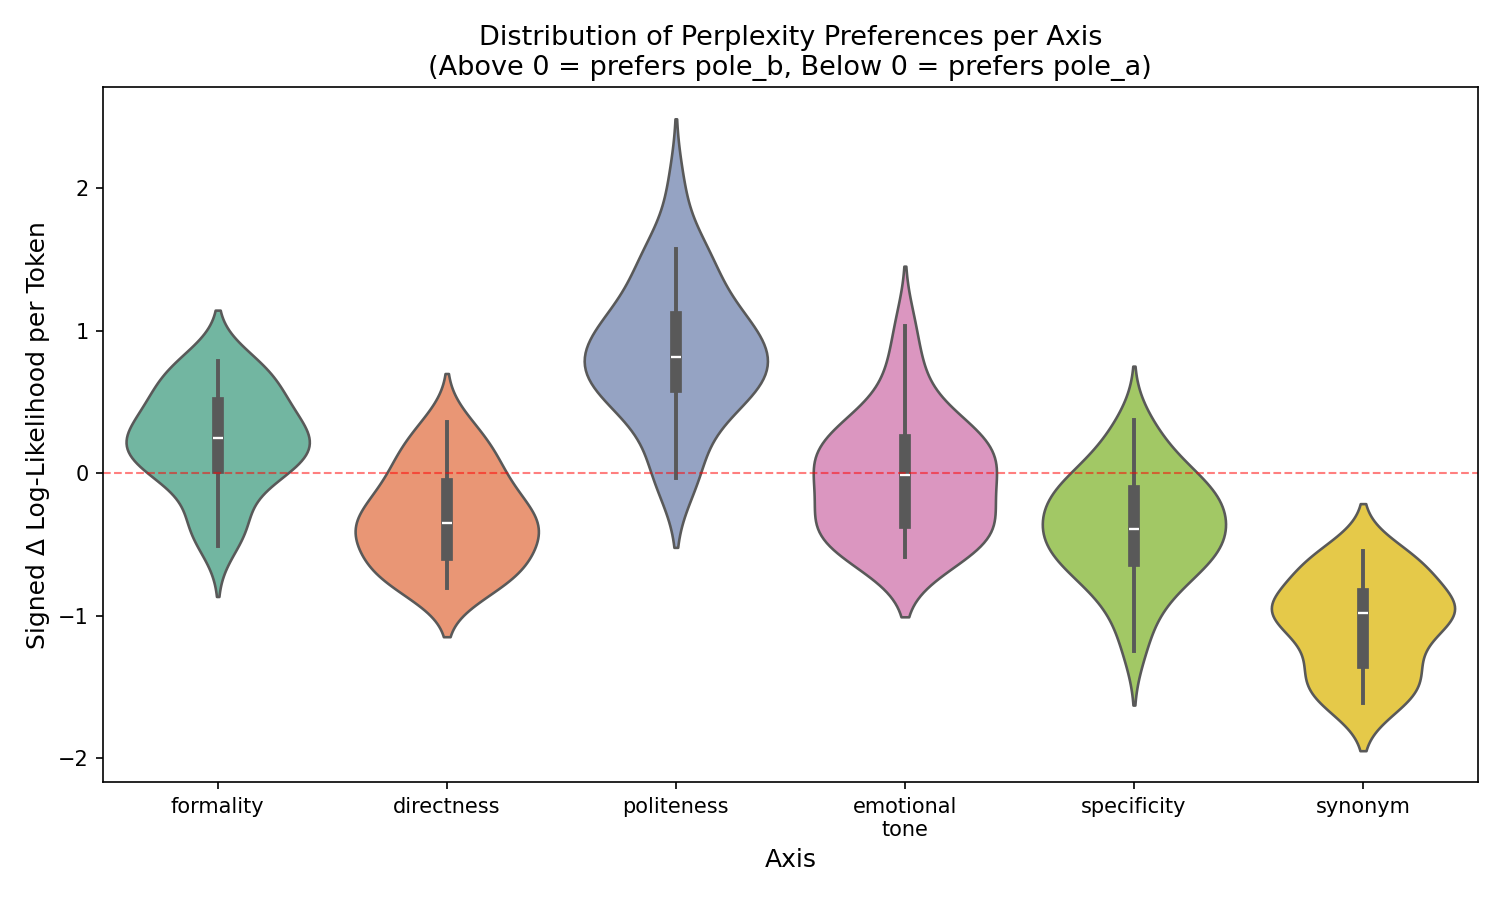
\includegraphics[width=0.95\linewidth]{figures/distribution_violin.png}
    \caption{Violin plots of signed $\dloglik$ across 30 scenarios for each axis (\qwenseven). Politeness shows a tight, positive distribution; emotional tone is centered near zero. The synonym control shows a uniformly negative distribution, confirming surface-level sensitivity.}
    \label{fig:violins}
\end{figure}

\subsection{Introspection vs.\ Behavioral Detection}
\label{sec:introspection_results}

\Tabref{tab:introspection} compares behaviorally detected axes (via perplexity sensitivity) against introspectively reported axes (via \gptfour self-report). Agreement holds for three of five axes (60\%).

\begin{table}[t]
    \centering
    \caption{Comparison of behavioral detection (perplexity sensitivity on \qwenseven) vs.\ introspective self-report (\gptfour). Introspection rate: fraction of scenarios where the model mentions the axis. Agreement holds for 3/5 axes.}
    \begin{tabular}{@{}lrrccl@{}}
        \toprule
        \textbf{Axis} & \textbf{Introsp.\ rate} & \textbf{Consistency} & \textbf{PPL det.?} & \textbf{Introsp.?} & \textbf{Match?} \\
        \midrule
        Formality      & 76.7\% & 0.533 & \checkmark & \checkmark & agree \\
        Directness     &  6.7\% & 0.600 & \checkmark & ---        & \textbf{differ} \\
        Politeness     & 63.3\% & 0.933 & \checkmark & \checkmark & agree \\
        Emot.\ tone    & 53.3\% & 0.067 & ---        & \checkmark & \textbf{differ} \\
        Specificity    & 83.3\% & 0.733 & \checkmark & \checkmark & agree \\
        \bottomrule
    \end{tabular}
    \label{tab:introspection}
\end{table}

The two disagreements are informative. \textbf{Directness} represents a \emph{blind spot}: the model strongly defaults to indirect, hedged responses ($d{=}0.94$) but almost never self-reports directness as a variable it considered (6.7\%). The model's hedging behavior appears deeply embedded in its generation prior, below the threshold of introspective access. \textbf{Emotional tone} represents \emph{performative consideration}: the model frequently claims to consider tone (53.3\%) but shows no consistent behavioral preference. This could reflect genuine per-scenario deliberation (without a stable default) or learned tendency to mention ``tone'' as a socially expected response. \Figref{fig:introspection} visualizes this comparison.

\begin{figure}[t]
    \centering
    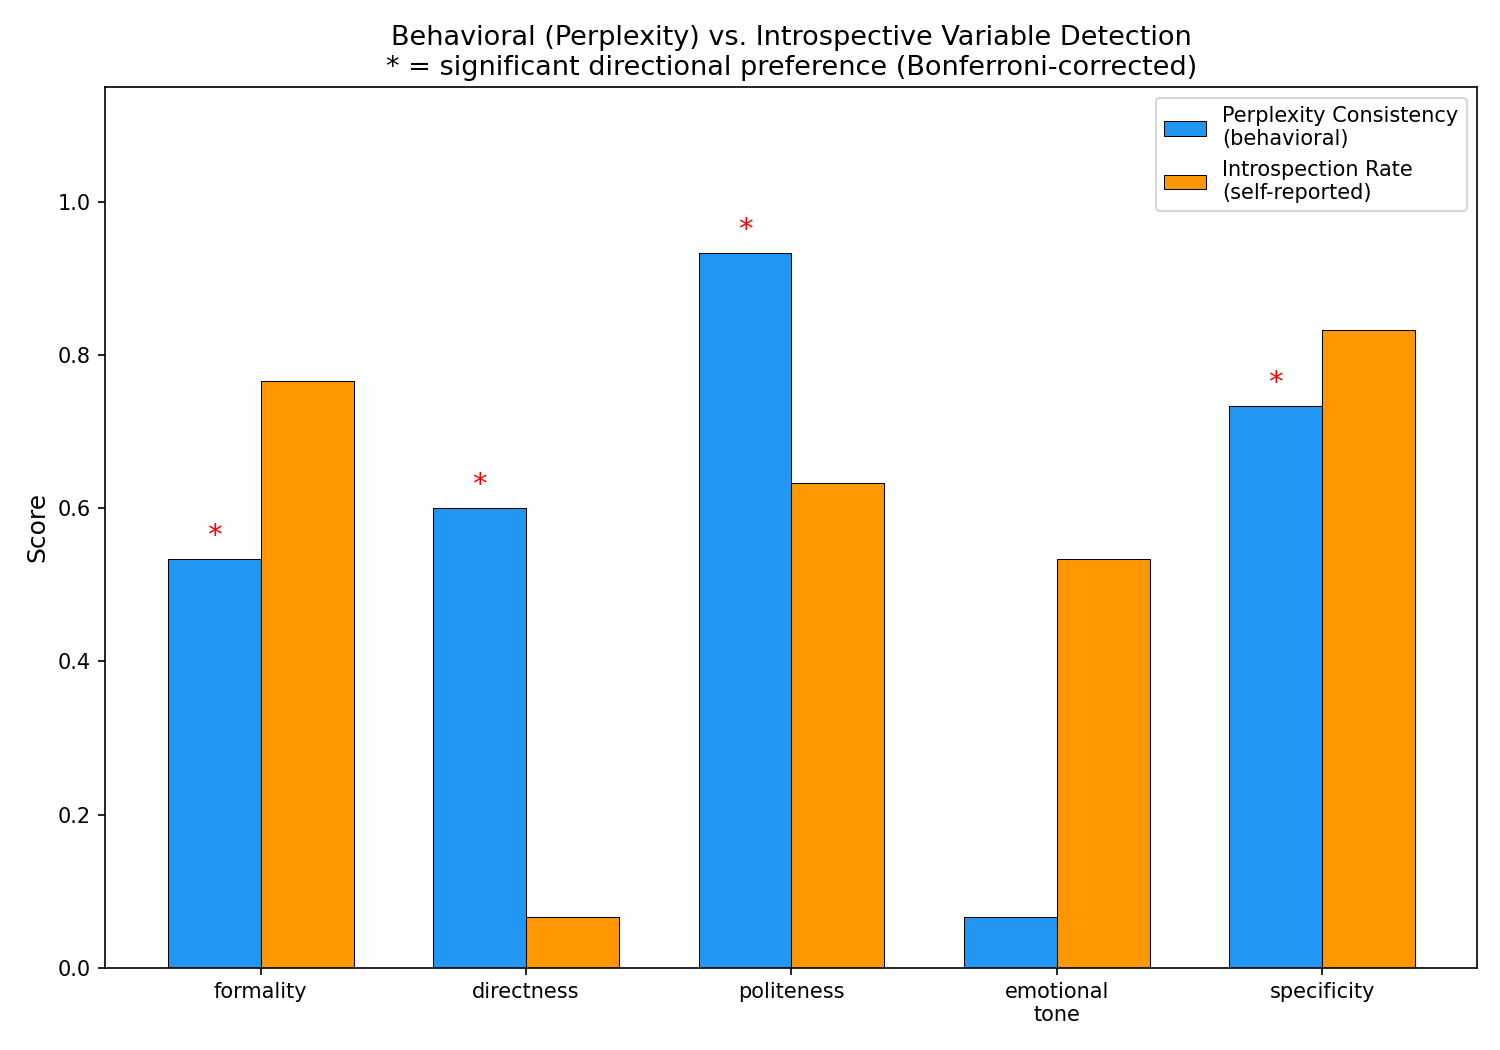
\includegraphics[width=0.95\linewidth]{figures/introspection_vs_behavioral.png}
    \caption{Behavioral vs.\ introspective detection of pragmatic variables. The two methods agree on formality, politeness, and specificity but diverge on directness (behavioral only) and emotional tone (introspective only).}
    \label{fig:introspection}
\end{figure}

\subsection{Cross-Model Replication}
\label{sec:cross_model}

\Tabref{tab:cross_model} compares effect sizes between \qwenseven and \qwenthree. All five axes show identical directional preferences across models, with a Spearman rank correlation of $\rho{=}1.0$ ($p{<}0.001$).

\begin{table}[t]
    \centering
    \caption{Cross-model comparison of effect sizes (Cohen's $d$). Both models show identical preference directions and the same ranking by $|d|$. Spearman $\rho{=}1.0$.}
    \begin{tabular}{@{}lrrl@{}}
        \toprule
        \textbf{Axis} & \textbf{\qwenseven $d$} & \textbf{\qwenthree $d$} & \textbf{Same dir.?} \\
        \midrule
        Politeness   & $+1.81$ & $+2.18$ & \checkmark \\
        Specificity  & $-1.02$ & $-1.36$ & \checkmark \\
        Directness   & $-0.94$ & $-0.59$ & \checkmark \\
        Formality    & $+0.68$ & $+0.99$ & \checkmark \\
        Emot.\ tone  & $-0.08$ & $-0.02$ & \checkmark \\
        \bottomrule
    \end{tabular}
    \label{tab:cross_model}
\end{table}

The smaller model shows slightly stronger effects for politeness ($d{=}2.18$ vs.\ $1.81$), specificity ($d{=}1.36$ vs.\ $1.02$), and formality ($d{=}0.99$ vs.\ $0.68$), while the larger model shows a stronger directness effect ($d{=}0.94$ vs.\ $0.59$). Both models show negligible emotional tone effects. \Figref{fig:cross_model} visualizes this agreement.

\begin{figure}[t]
    \centering
    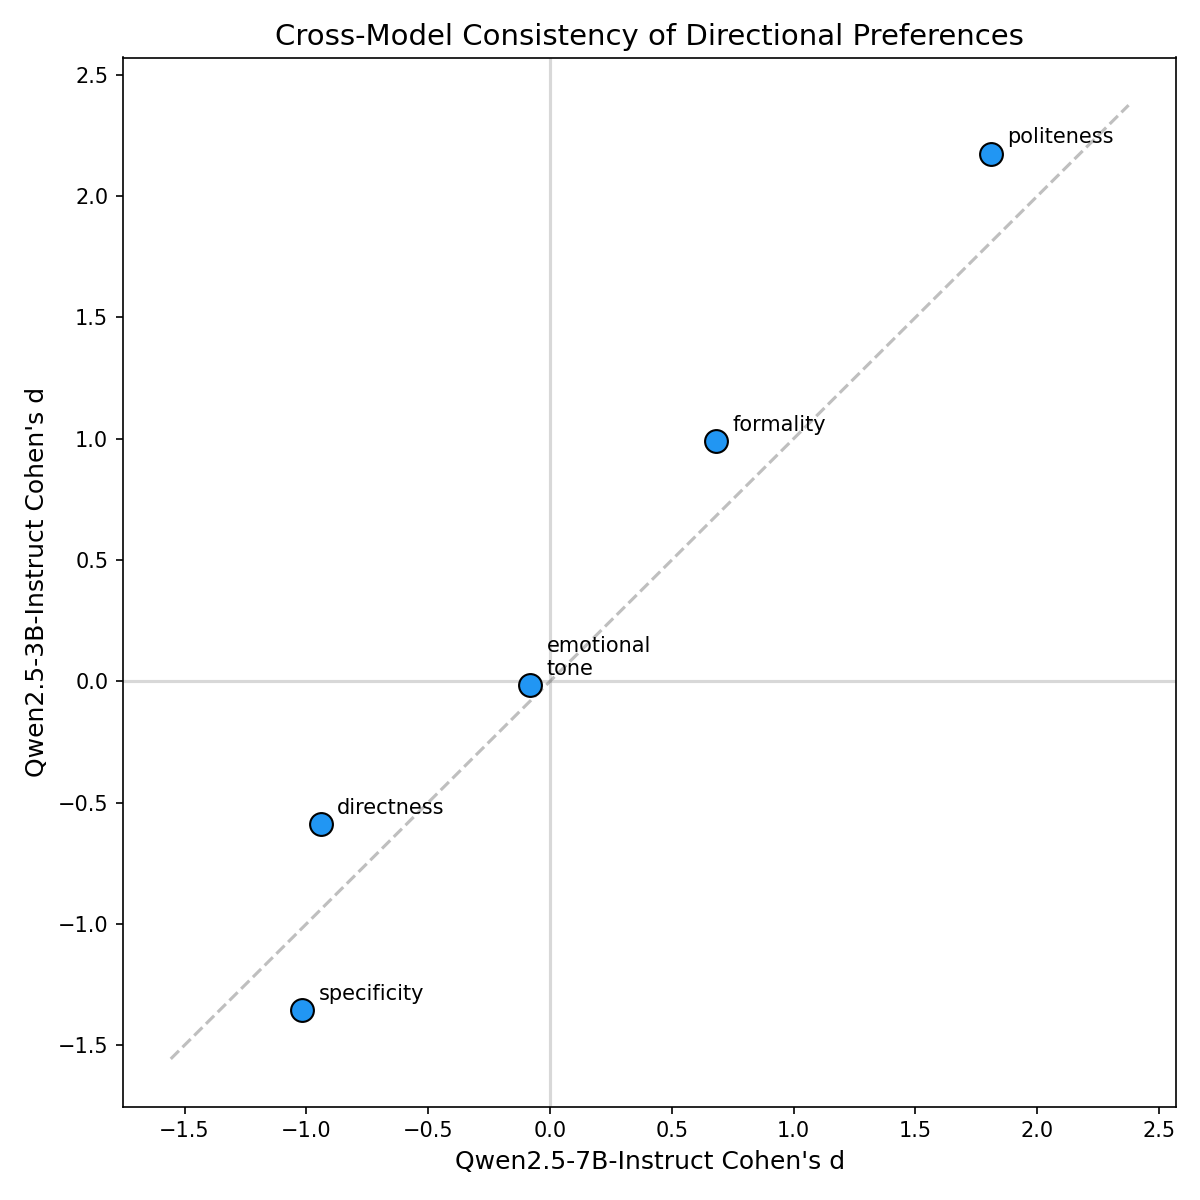
\includegraphics[width=0.75\linewidth]{figures/cross_model_comparison.png}
    \caption{Effect sizes for \qwenseven vs.\ \qwenthree. Points fall near the diagonal, confirming cross-size replication. Spearman $\rho{=}1.0$.}
    \label{fig:cross_model}
\end{figure}
